\documentclass{beamer}
\usepackage[utf8]{inputenc}
\usepackage[]{amsmath}
\usepackage{graphicx}
\usepackage{physics}
\usepackage{subcaption} % package pour faire des subfigures
\usepackage{multirow} % package pour multirow/multicolumn
\usepackage{booktabs} % package pour top/mid/bottom rule
\usepackage{tcolorbox} % toujours plus de boites
\usepackage[backend=biber]{biblatex}


\addbibresource{Biblio_dbl_quantum.bib}

%\bibliographystyle{stylename}
%\bibliography{Biblio_dbl_quantum}

\title{Group meeting : Cross-relaxation with NV centers ensemble in diamond}
%\author{Clément Pellet-Mary\\ Laboratoire de physique de l'ENS\\ \textit{ENS, Paris}}
\date\today

\mode<presentation> {\usetheme{Rochester}}

\begin{document}
\begin{frame}
\maketitle
\end{frame}
\begin{frame}{Outline}
\tableofcontents
\end{frame}
\section{(Quick) Reminder on NV center}
\begin{frame}{Outline}
\tableofcontents[currentsection]
\end{frame}
\begin{frame}{NV$^-$ spin in the fundamental electronic state}
\centering
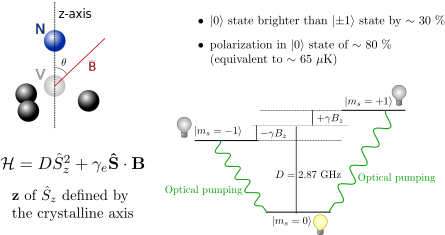
\includegraphics[width=\textwidth,height=\textheight,keepaspectratio]{slide_3_niveaux}
\end{frame}
\begin{frame}{Principle of CW ODMR}
\centering
\includegraphics[width=\textwidth,height=0.9\textheight,keepaspectratio]{shéma lock in ESR}
\end{frame}
\section{Dipolar interaction and spin lifetime}
\begin{frame}{Outline}
\tableofcontents[currentsection]
\end{frame}
\begin{frame}{Today's goal : understand the PL dip in zero-field}
\centering
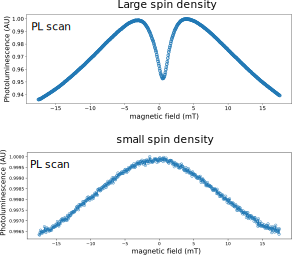
\includegraphics[width=\textwidth,height=0.9\textheight,keepaspectratio]{Slide 1}
\end{frame}
\begin{frame}{Why does it matter ?}
\begin{itemize}
\item The concentration of NV$^-$ centers (while maintaining good spectral properties) is increasing.
\item Magnetometry in low field is already hard with standard techniques.
\item The dip itself can be used to perform low-field, microwave-less magnetometry.
\end{itemize}
\end{frame}
\begin{frame}{Link between the PL and the spin T1}
\centering
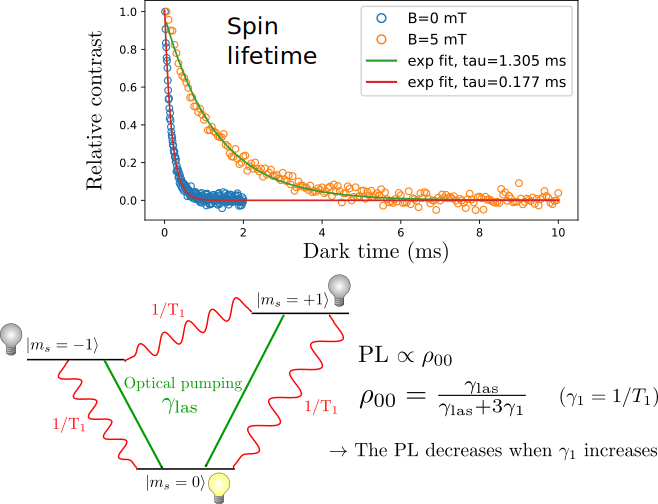
\includegraphics[width=\textwidth,height=0.9\textheight,keepaspectratio]{Explication T1 PL}
\end{frame}
\begin{frame}{Spin relaxation amplified by dipolar coupling}
See animation
\end{frame}
\begin{frame}{Dipolar interaction should not modify the total spin polarization...}
\centering
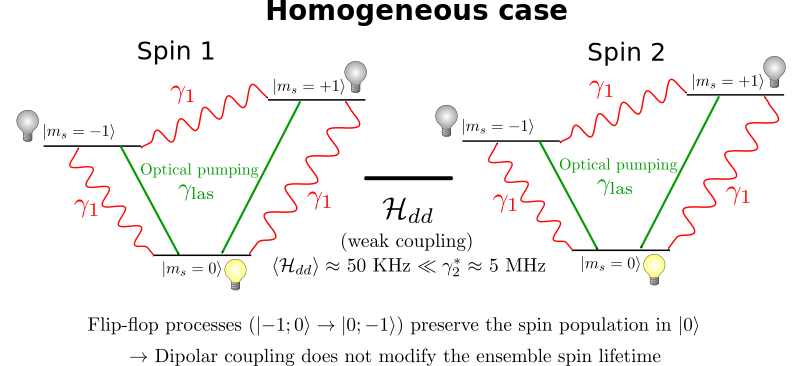
\includegraphics[width=\textwidth,height=0.9\textheight,keepaspectratio]{Flip flop inhomogénités}
\end{frame}
\begin{frame}{...except with inhomogeneities }
\centering
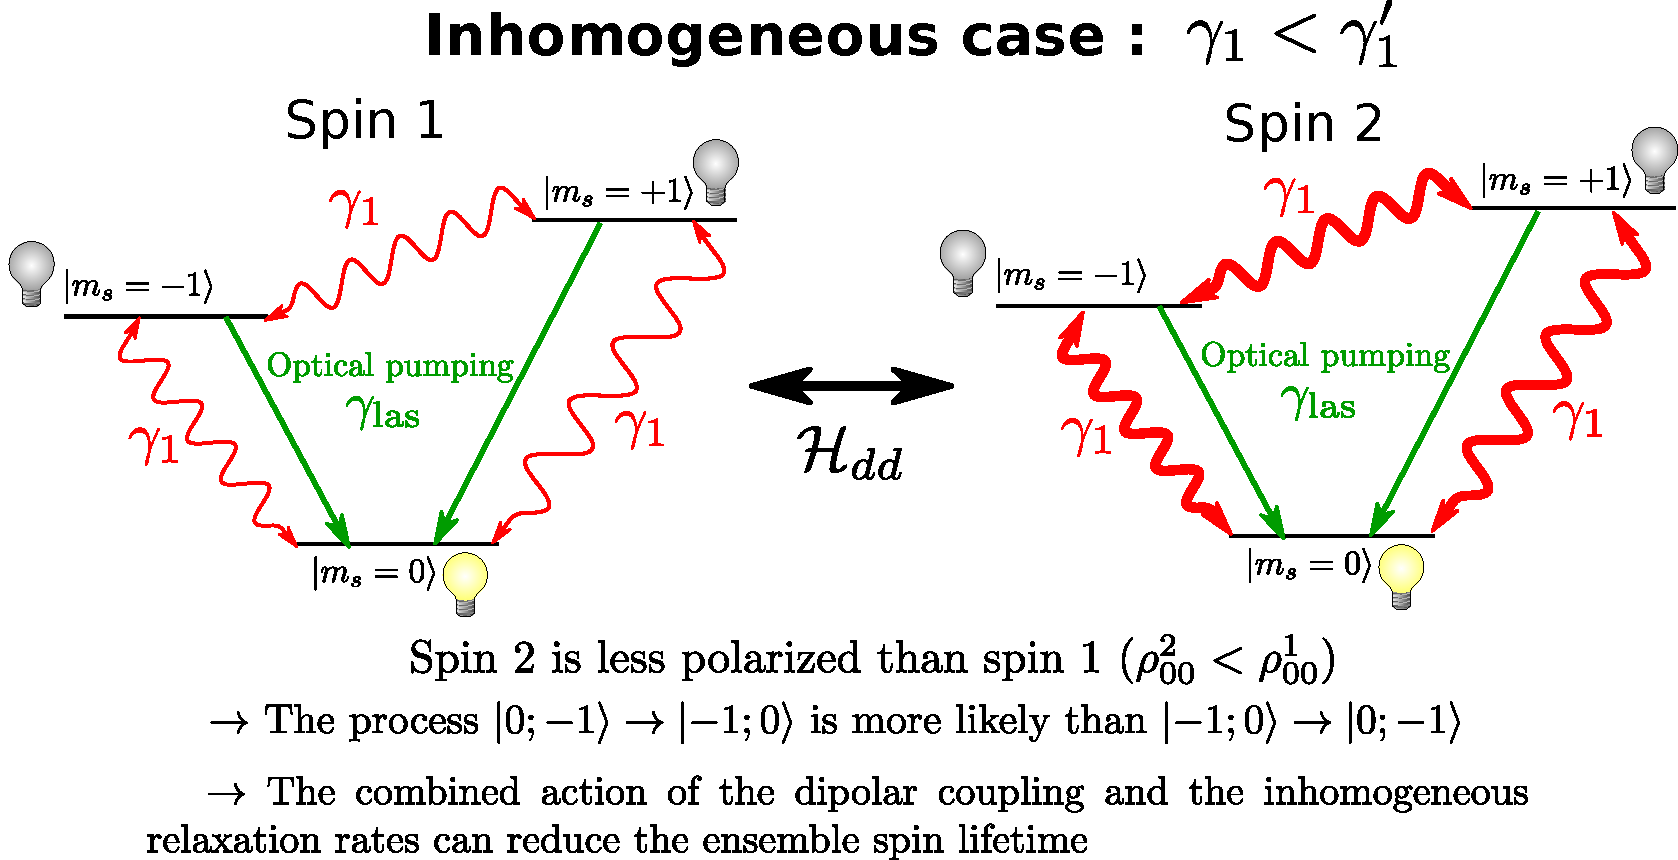
\includegraphics[width=\textwidth,height=0.9\textheight,keepaspectratio]{Flip flop inhomogénités 2}
\end{frame}
\section{The fluctuator model}
\begin{frame}{Outline}
\tableofcontents[currentsection]
\end{frame}
\begin{frame}{Theoretical frame : the fluctuator model}
\centering
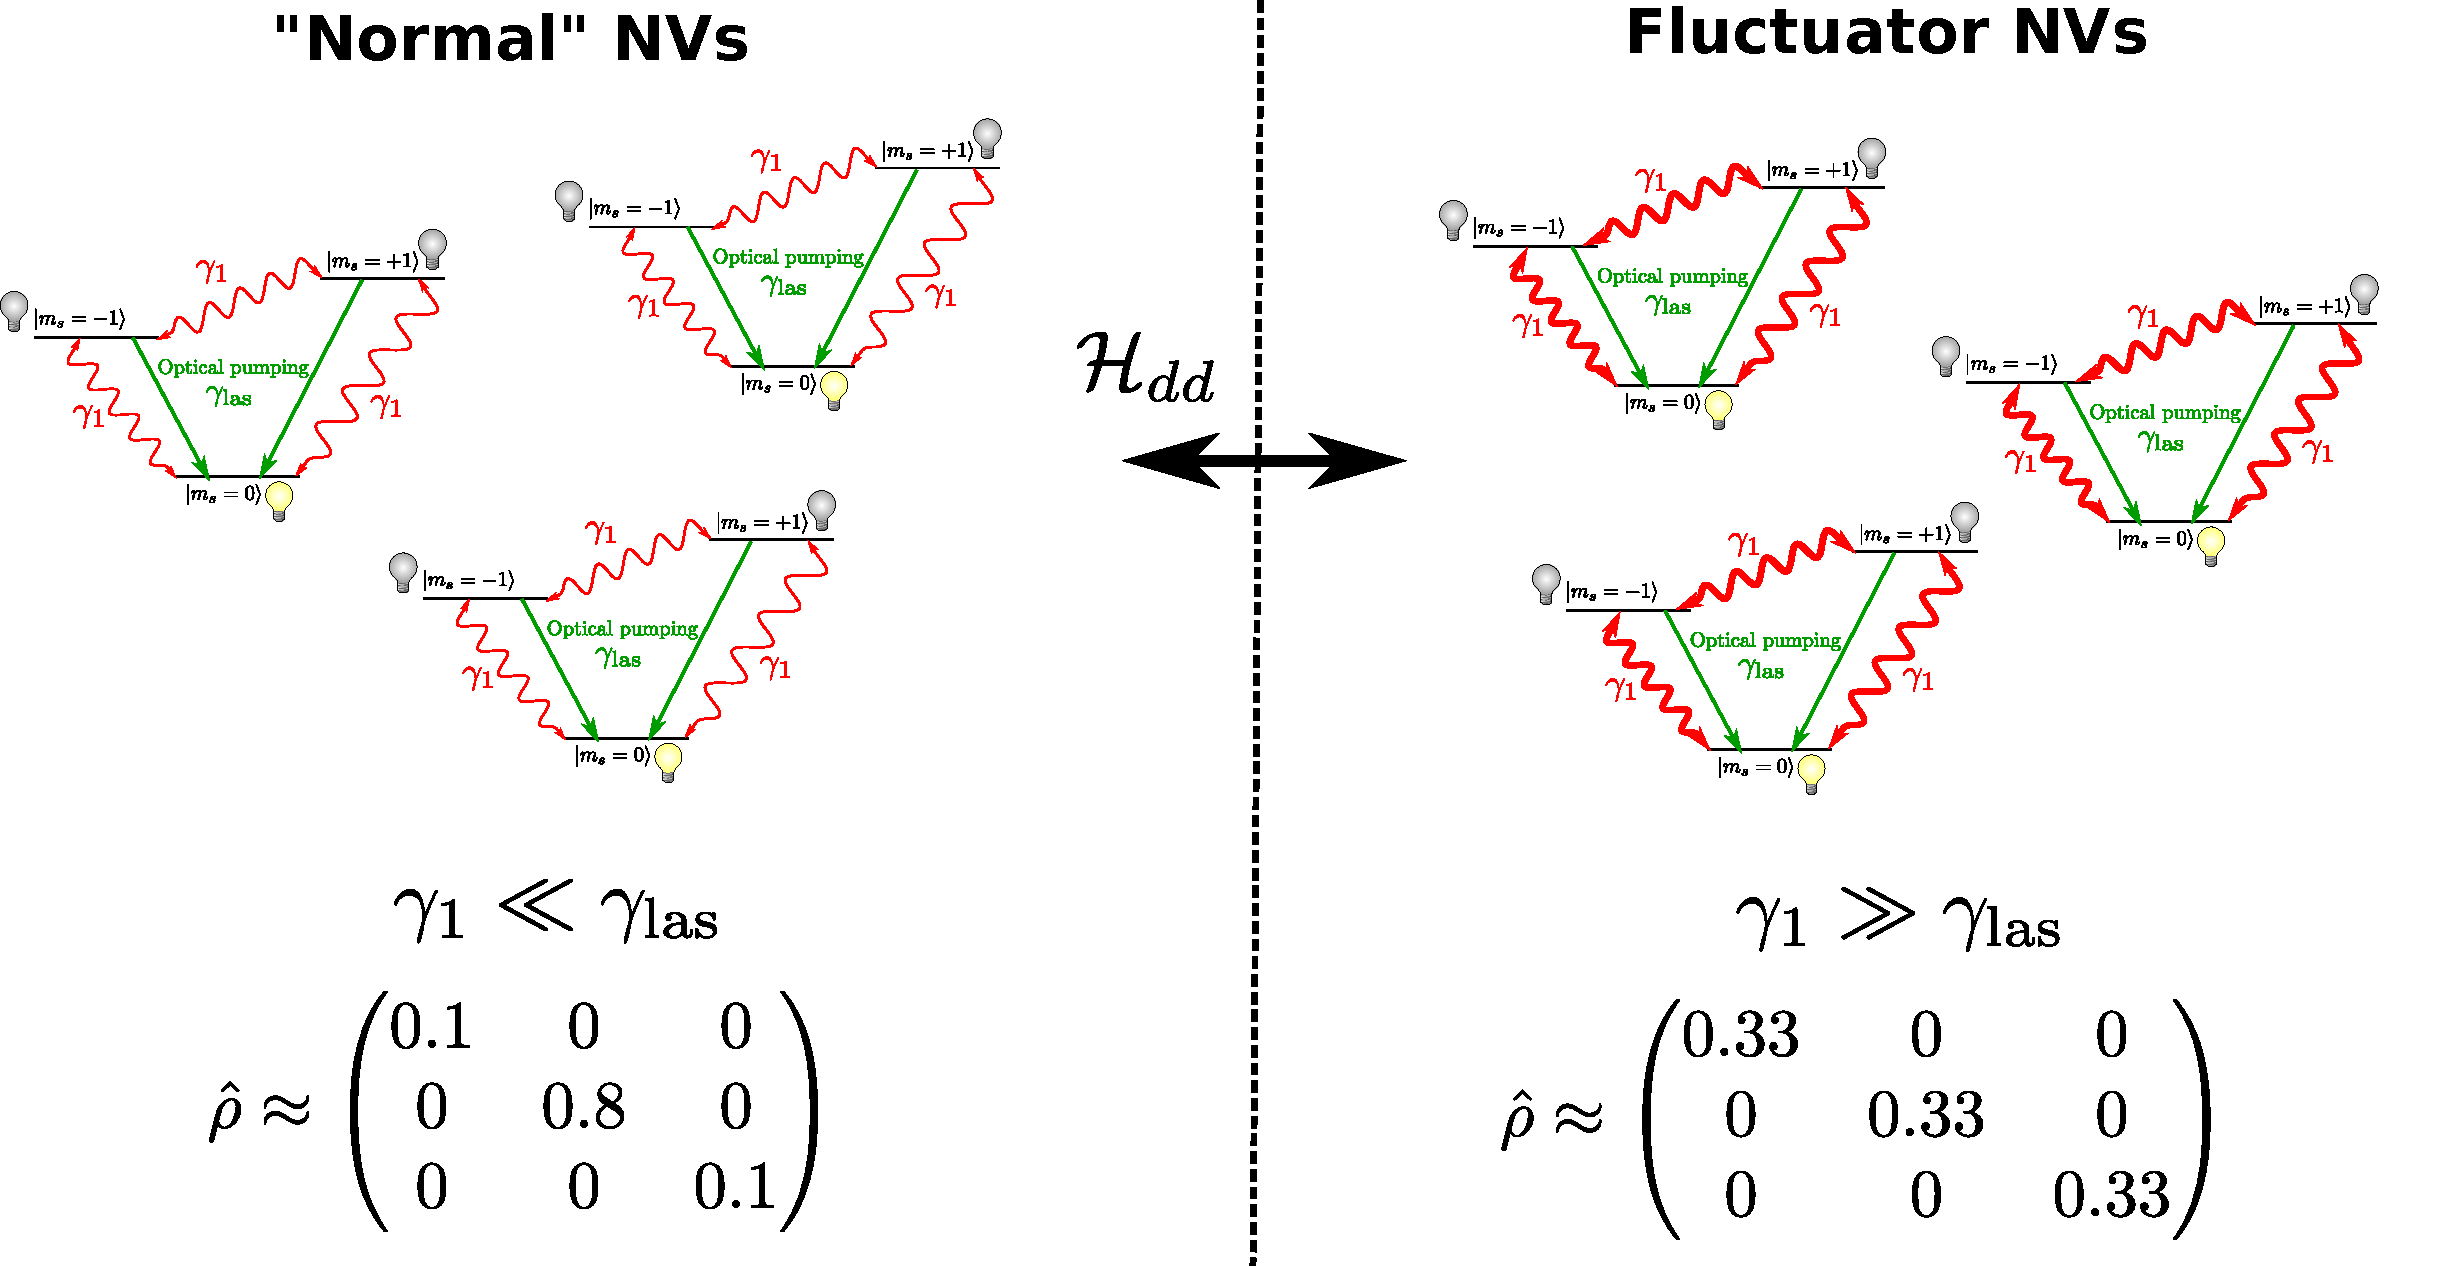
\includegraphics[width=\textwidth,height=0.9\textheight,keepaspectratio]{NV Vs Fluct}
\end{frame}
\begin{frame}{The dipole-dipole Hamiltonian}
\begin{center}
\includegraphics[scale=0.4]{Shéma dipole-dipole}
\end{center}

\begin{equation*}
  \mathcal{H}_{dd}=-\frac{\mu_0 \gamma_1 \gamma_2 \hbar ^2}{4 \pi r^3}[3(\mathbf{\hat{S}_1}\cdot \mathbf{u})(\mathbf{\hat{S}_2}\cdot \mathbf{u})-\mathbf{\hat{S}_1}\cdot \mathbf{\hat{S}_2}]
  \end{equation*}
  
  Every matrix element $\matrixel{i;\alpha}{\mathcal{H}_{dd}}{j;\beta}$ can be written as $\xi(\lVert \vec r \rVert)  \eta (\vec u)$ 
  
  \bigskip
  Example : $\matrixel{0;-1}{\mathcal{H}_{dd}}{-1;0}$ is the matrix element for a flip-flop process
\end{frame}
\begin{frame}{$\mathcal{H}_{dd}$ for two aligned spin}
In the magnetic basis $(\ket{-1},\ket{0},\ket{+1}) \otimes (\ket{-1},\ket{0},\ket{+1})$ :

\begin{align}
  \mathcal{H}_{dd}\propto &(\frac{3}{2}(n_x^2+n_y^2)-1)\left[\op{0;+1}{+1;0}+\op{-1;0}{0;-1} + h.c. \right]\\
  &+\frac{3}{2}(n_x^2-n_y^2+i2n_x n_y)\left[\op{0;+1}{-1;0}+\op{+1;0}{0;-1}\right]\\
  &+\frac{3}{2}(n_x^2-n_y^2-i2n_x n_y)\left[\op{0;-1}{+1;0}+\op{-1;0}{0;+1}\right]\\
  &+(3n_z^2-1)\hat{S_z^1}\hat{S_z^2}\\
  &+\mathcal{H}_{\mathrm{other}}
  \end{align}

Example : $\eta_{\mathrm{flip-flop}}=\frac{3}{2}(n_x^2+n_y^2)-1)$
\end{frame}

\begin{frame}{The fluctuator model : calculation steps}
\begin{itemize}
\item Decay rate induced by a single fluctuator on a single NV : $$
\Gamma_{ij}=\sum_{\alpha,\beta} \lvert \matrixel{i,\alpha}{\mathcal{H}_{dd}}{j,\beta} \rvert ^2 \frac{\gamma_f}{(\omega_{ij}-\omega_{\beta \alpha})^2 + \gamma_f^2}
$$
\pause
\item Each NV will see a total decay rate $$\gamma = \sum_\mathrm{fluct} \Gamma_{ij}(\vec r)$$
\end{itemize}
\end{frame}
\begin{frame}{The fluctuator model : calculation steps}
\begin{itemize}
\item We can compute the distribution of these individual decay rates $\gamma$ :
\begin{align*}
\rho(\gamma)&=\int \left\{ d_{\mathrm{fluct}} \right\} \delta \left( \gamma - \sum_\mathrm{fluct} \Gamma_{ij}(\vec r) \right) \\
&=\frac{e^{-1/(4\gamma T)}}{\sqrt{4 \pi \gamma^3 T}}
\end{align*}


\pause
\item The measured lifetime will be averaged over all the NVs :
$$
PL(t) = \int e^{-\gamma t} \rho(\gamma) d\gamma = e^{-\sqrt{t/T}}
$$
\end{itemize}
\end{frame}
\begin{frame}{The fluctuator model : calculation steps}
Where :
$$
T \equiv \left( \frac{4 \pi n_f J_0 \bar \eta}{3} \right) ^2 \frac{\pi}{\gamma_f}
$$

With :
\begin{itemize}
\item $n_f$ is the fluctuator density
\item $\gamma_f$ is the fluctuator decay rate
\end{itemize}

and :
$$
 \bar \eta \equiv \frac{1}{4} \sum_{\mathrm{classes}} \frac{\gamma_f^2}{(\omega_{\mathrm{NV}}-\omega_{\mathrm{fluct}})^2 + \gamma_f^2} \int_{\theta , \phi} \lvert \eta(\theta , \phi) \rvert \dd \Omega 
$$
\end{frame}

\begin{frame}{Examples}

%\begin{align*}
% \bar \eta &= \frac{1}{4} \int_{\theta , \phi} \lvert \eta(\theta , \phi) \rvert \dd \Omega \\
% &= \frac{1}{4}\times 0.3849
%\end{align*}
%
%\begin{align*}
% \bar \eta &= \frac{1}{4} \int_{\theta , \phi} \lvert \eta(\theta , \phi) \rvert \dd \Omega + \frac{1}{4} \int_{\theta , \phi} \lvert \eta ' (\theta , \phi) \rvert \dd \Omega \\
% &= \frac{1}{4}*0.3849 + \frac{1}{4}*0.8328
%\end{align*}

\centering
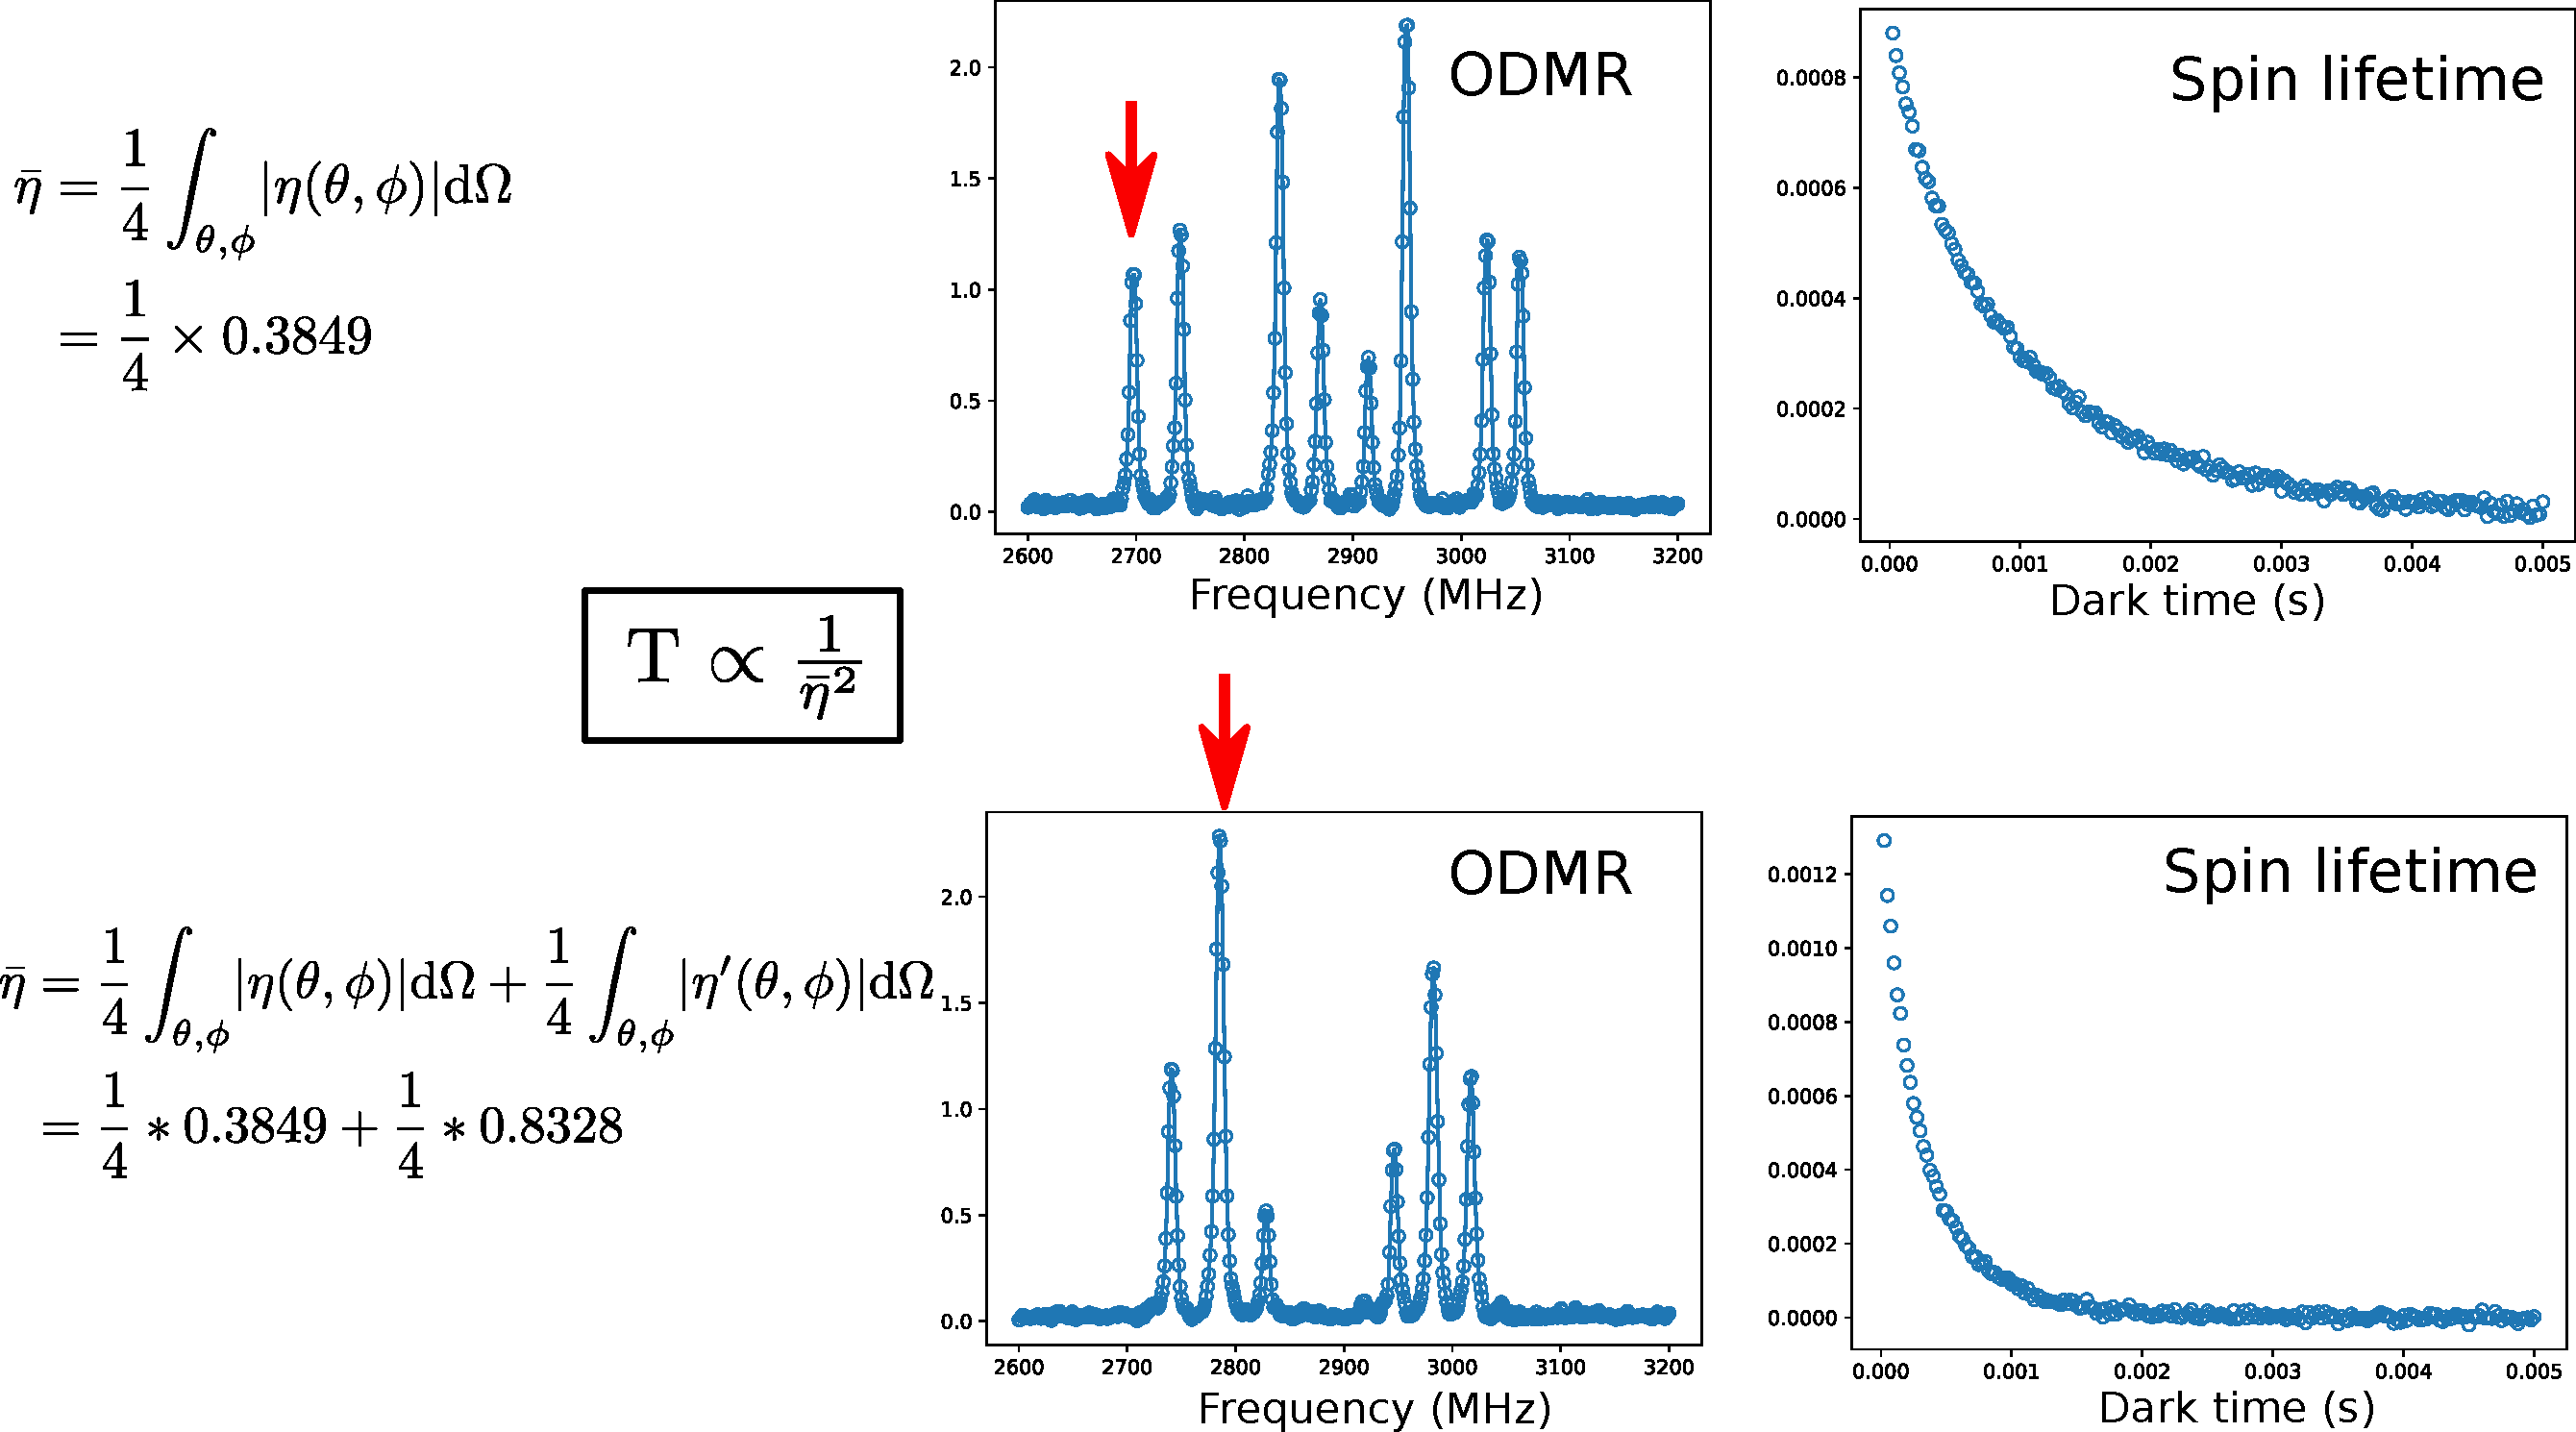
\includegraphics[width=\textwidth,height=0.9\textheight,keepaspectratio]{Exemple fluct 121 1x4}
\end{frame}

\begin{frame}{Non-trivial prediction of the model}
\centering
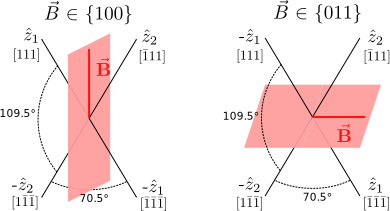
\includegraphics[width=\textwidth,height=0.9\textheight,keepaspectratio]{121 VS 22 shéma}
\end{frame}
\begin{frame}{Non-trivial prediction of the model}
\centering
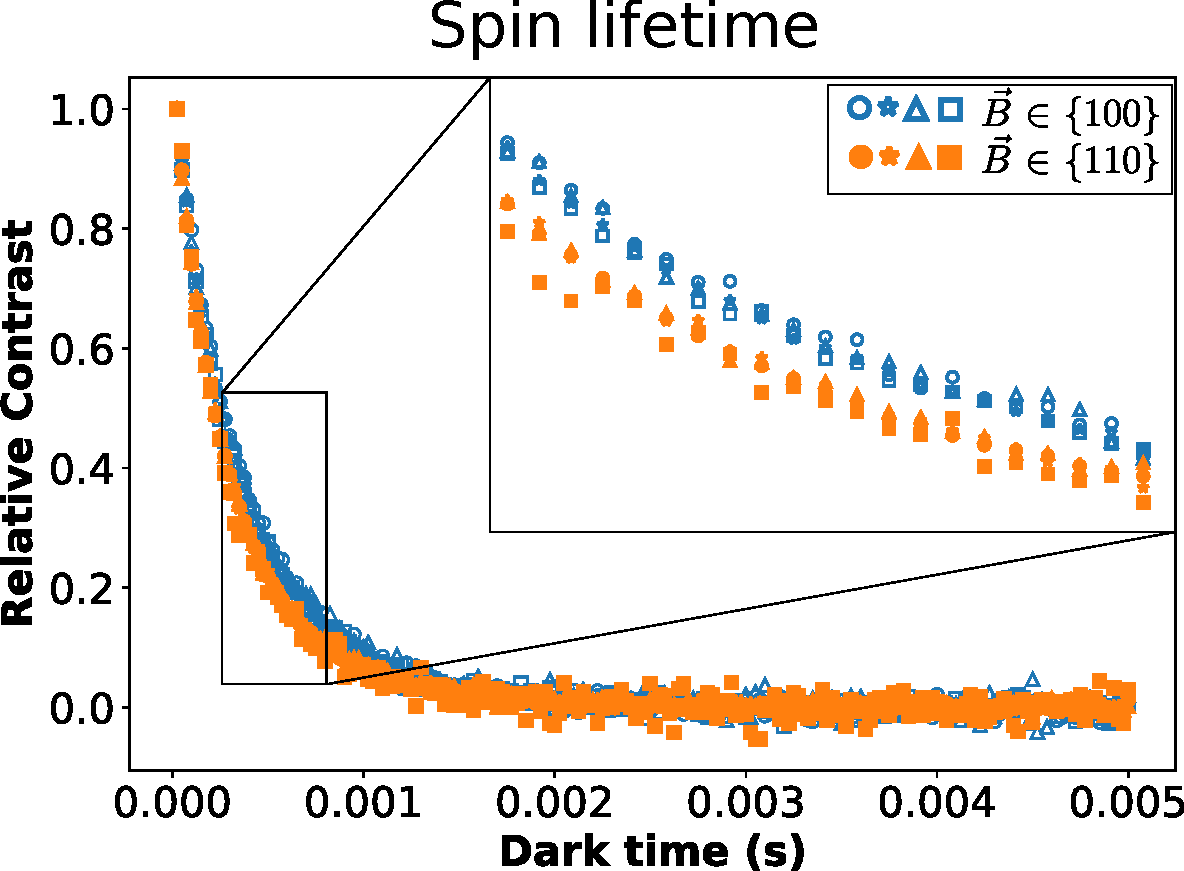
\includegraphics[width=\textwidth,height=0.9\textheight,keepaspectratio]{121 Vs 22 combined}
\end{frame}
\section{The reasons behind the dip in zero-field}
\begin{frame}{Outline}
\tableofcontents[currentsection]
\end{frame}
\begin{frame}{The reasons behind the dip in zero-field}
\begin{center}
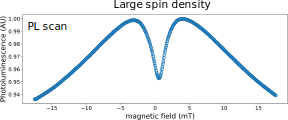
\includegraphics[width=.8\textwidth,height=0.9\textheight,keepaspectratio]{Scan PL random dir}
\end{center}

There are 3 parts, all linked to dipolar coupling :
\begin{enumerate}
\item The lift of the degeneracies between the four classes
\item The change of the eigenstates in the avoided crossing region
\item The double-flip terms in the dipolar Hamiltonian
\end{enumerate}
\end{frame}
\begin{frame}{1. The lift of the degeneracies}
\centering
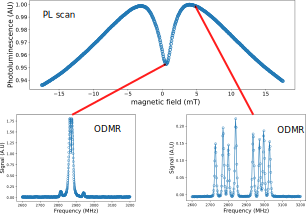
\includegraphics[width=\textwidth,height=0.9\textheight,keepaspectratio]{splitting degenerescence}
\end{frame}
\begin{frame}{But it is not the only reason}
\centering
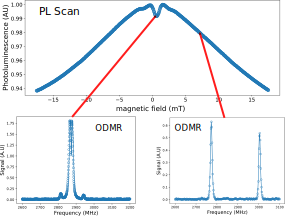
\includegraphics[width=\textwidth,height=0.9\textheight,keepaspectratio]{scan 100 slide}
\end{frame}
\begin{frame}{2. The change in eigenstates of $\mathcal{H}_0$}
%$$
%\mathcal{H}_0=\begin{pmatrix}
%D-\gamma_e B_z & \gamma_e B_x & d_\perp E_x \\
%\gamma_e B_x & 0 & \gamma_e B_x \\
%d_\perp E_x & \gamma_e B_x & D+\gamma_e B_z
%\end{pmatrix}
%$$
\centering
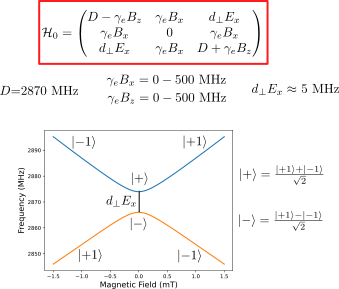
\includegraphics[width=\textwidth,height=0.9\textheight,keepaspectratio]{Coupled Basis}
\end{frame}
\begin{frame}{Dipolar Hamiltonian in the coupled basis}
\setcounter{equation}{0}
In the coupled basis $(\ket{-},\ket{0},\ket{+}) \otimes (\ket{-},\ket{0},\ket{+})$ :
\begin{align}
  \mathcal{H}_{dd}&=(3n_x^2-1)\left[\op{0;+}{+;0}+ h.c. \right]\\
  &+(3n_y^2-1)\left[\op{0;-}{-;0}+ h.c. \right]\\
  &+i3n_x n_y\left[\op{0;+}{-;0}+\op{+;0}{0;-} +h.c. \right]\\
  &+(3n_z^2-1)\left[\op{+;-}{-;+}+ h.c.\right]\\
  &+\mathcal{H}_{\mathrm{other}}
  \end{align}
  $\eta_{\mathrm{flip-flop}} = 3n_x^2-1$ or $3n_y^2-1 \neq \frac{3}{2}(n_x^2+n_y^2)-1$ 
  
  $\to \bar \eta_{\mathrm{flip-flop}}(\ket{\pm 1})=0.3849 < \bar \eta_{\mathrm{flip-flop}}(\ket{\pm})=0.7698$
\end{frame}
\begin{frame}{$\mathcal{H}_0$ under pure transverse field}
\centering
\includegraphics[width=\textwidth,height=0.9\textheight,keepaspectratio]{Base couplée : vec vs val}
\end{frame}
\begin{frame}{Experimental results with transverse field}
\centering
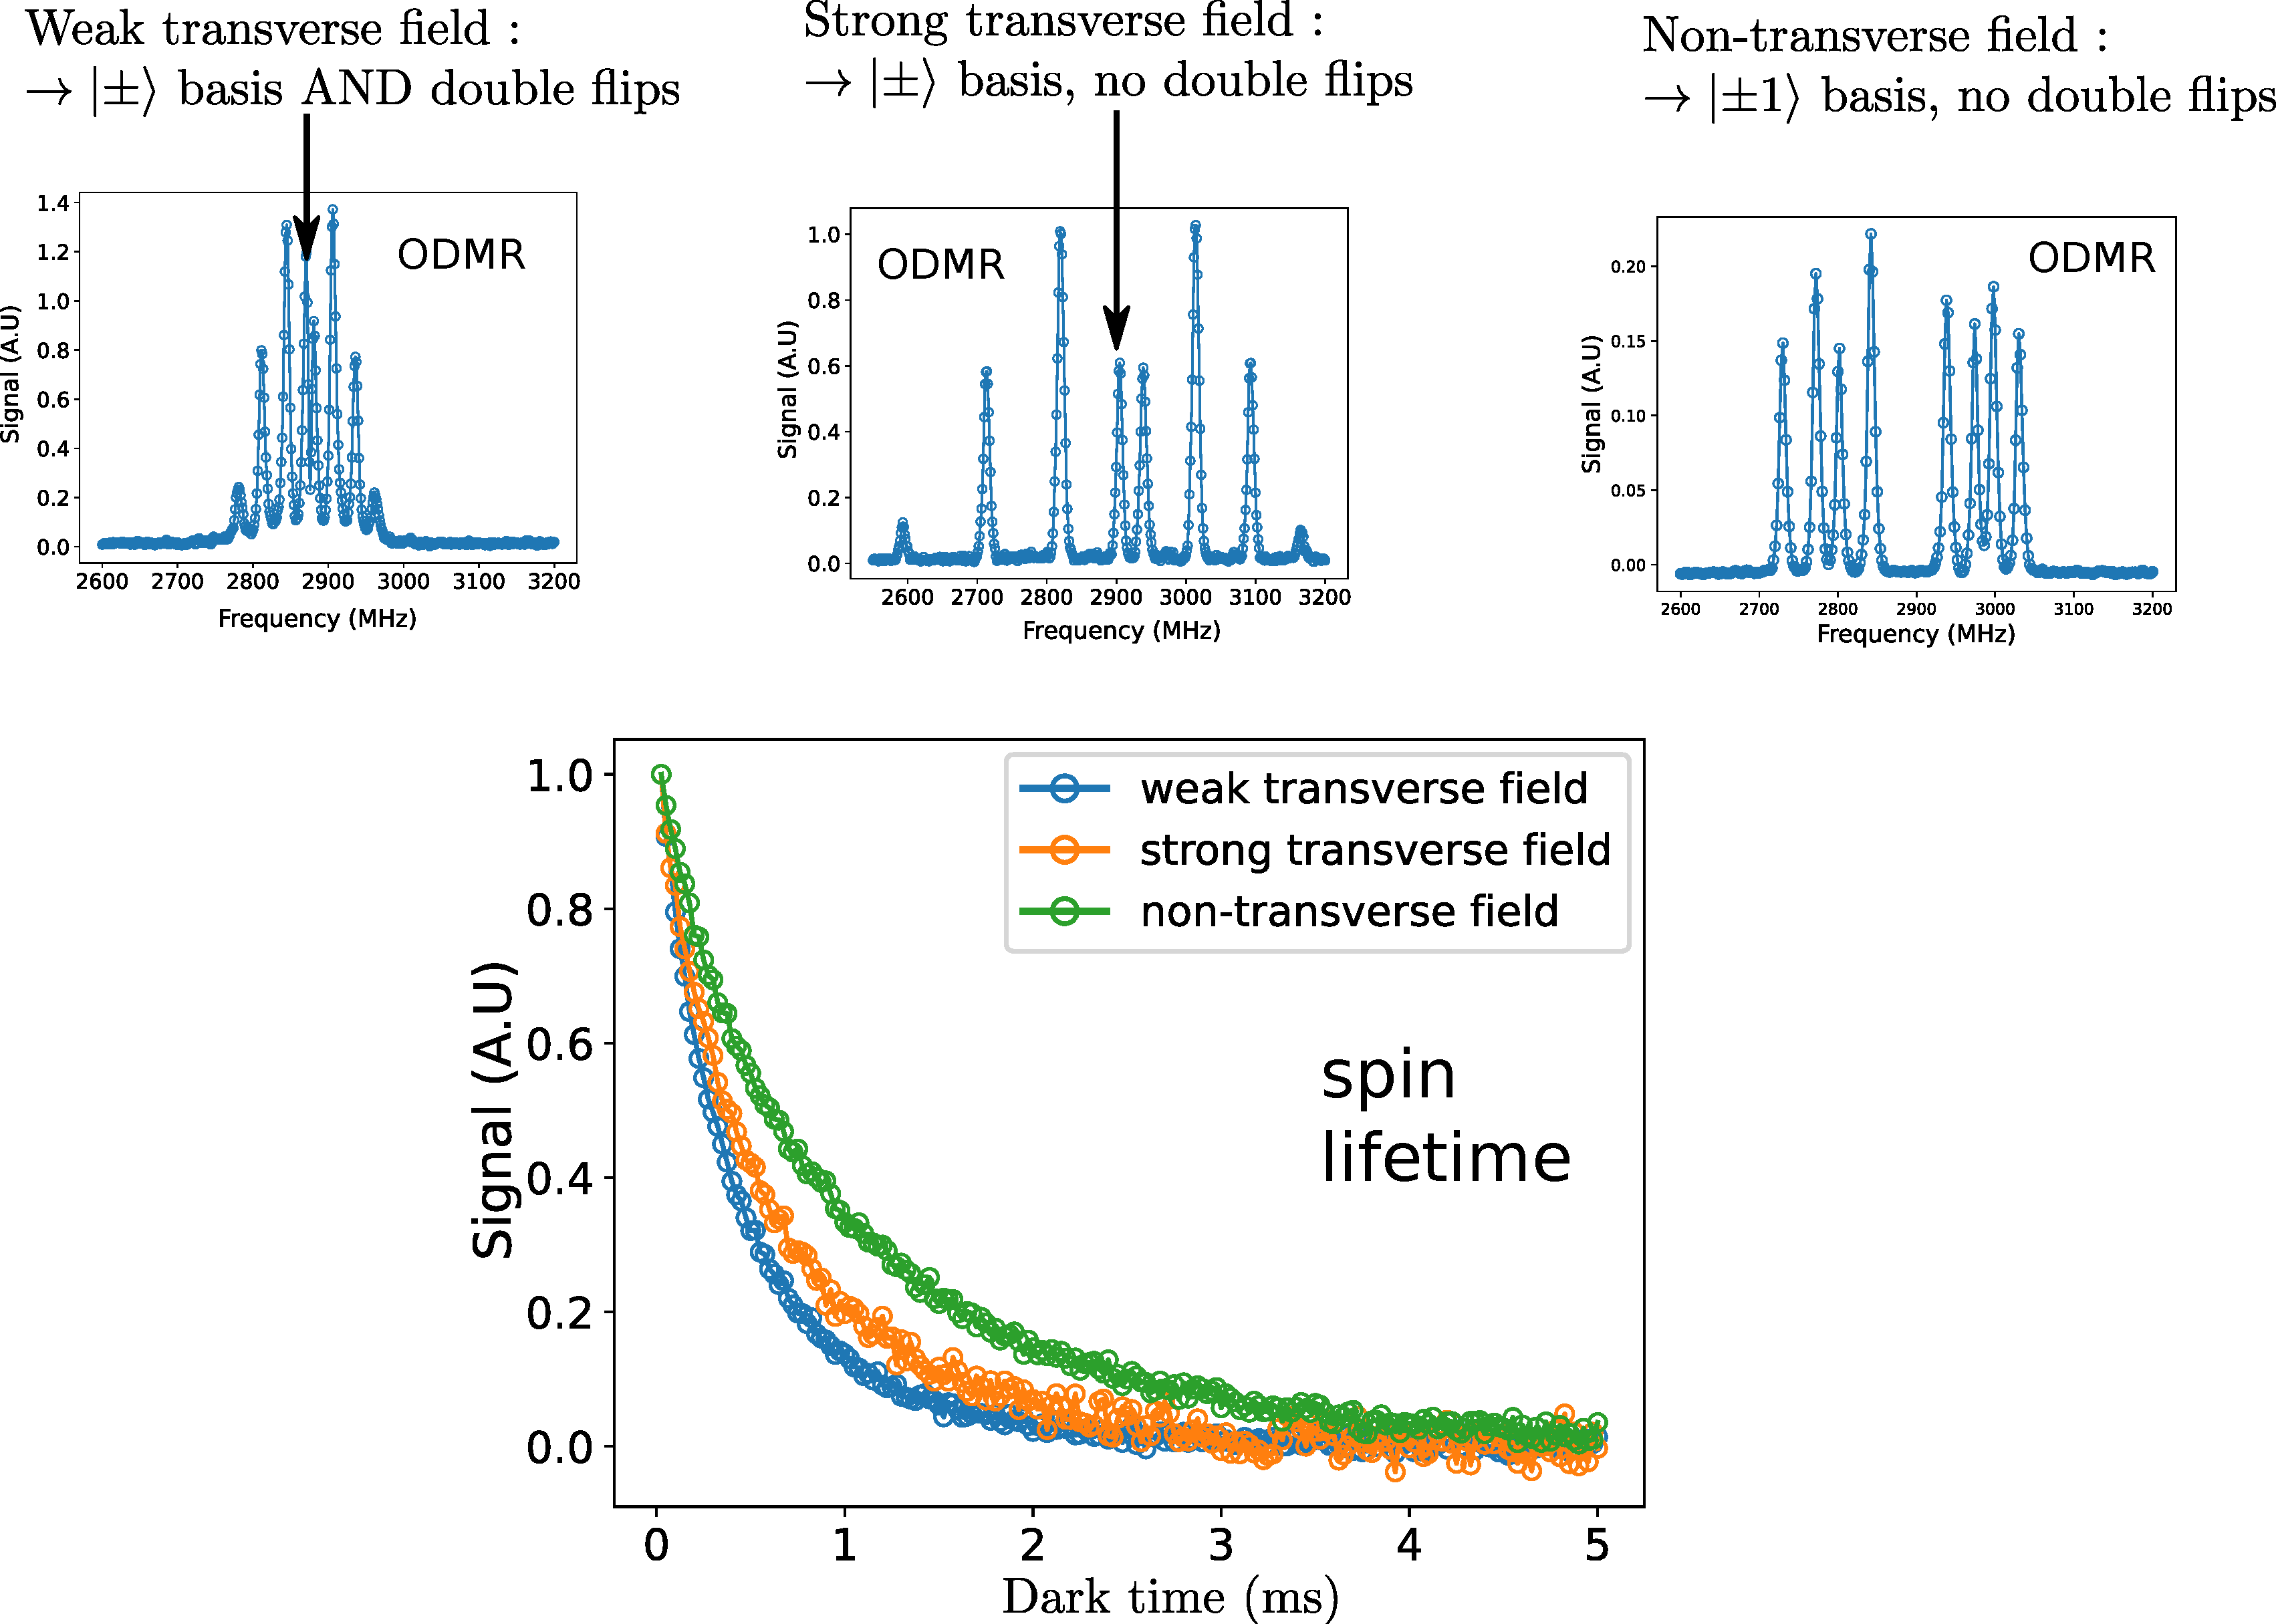
\includegraphics[width=\textwidth,height=0.9\textheight,keepaspectratio]{Champ transverse mesures}
\end{frame}
\section{Low-field Magnetometry}
\begin{frame}{Outline}
\tableofcontents[currentsection]
\end{frame}
\begin{frame}{Low field magnetometry experimental setup}
\centering
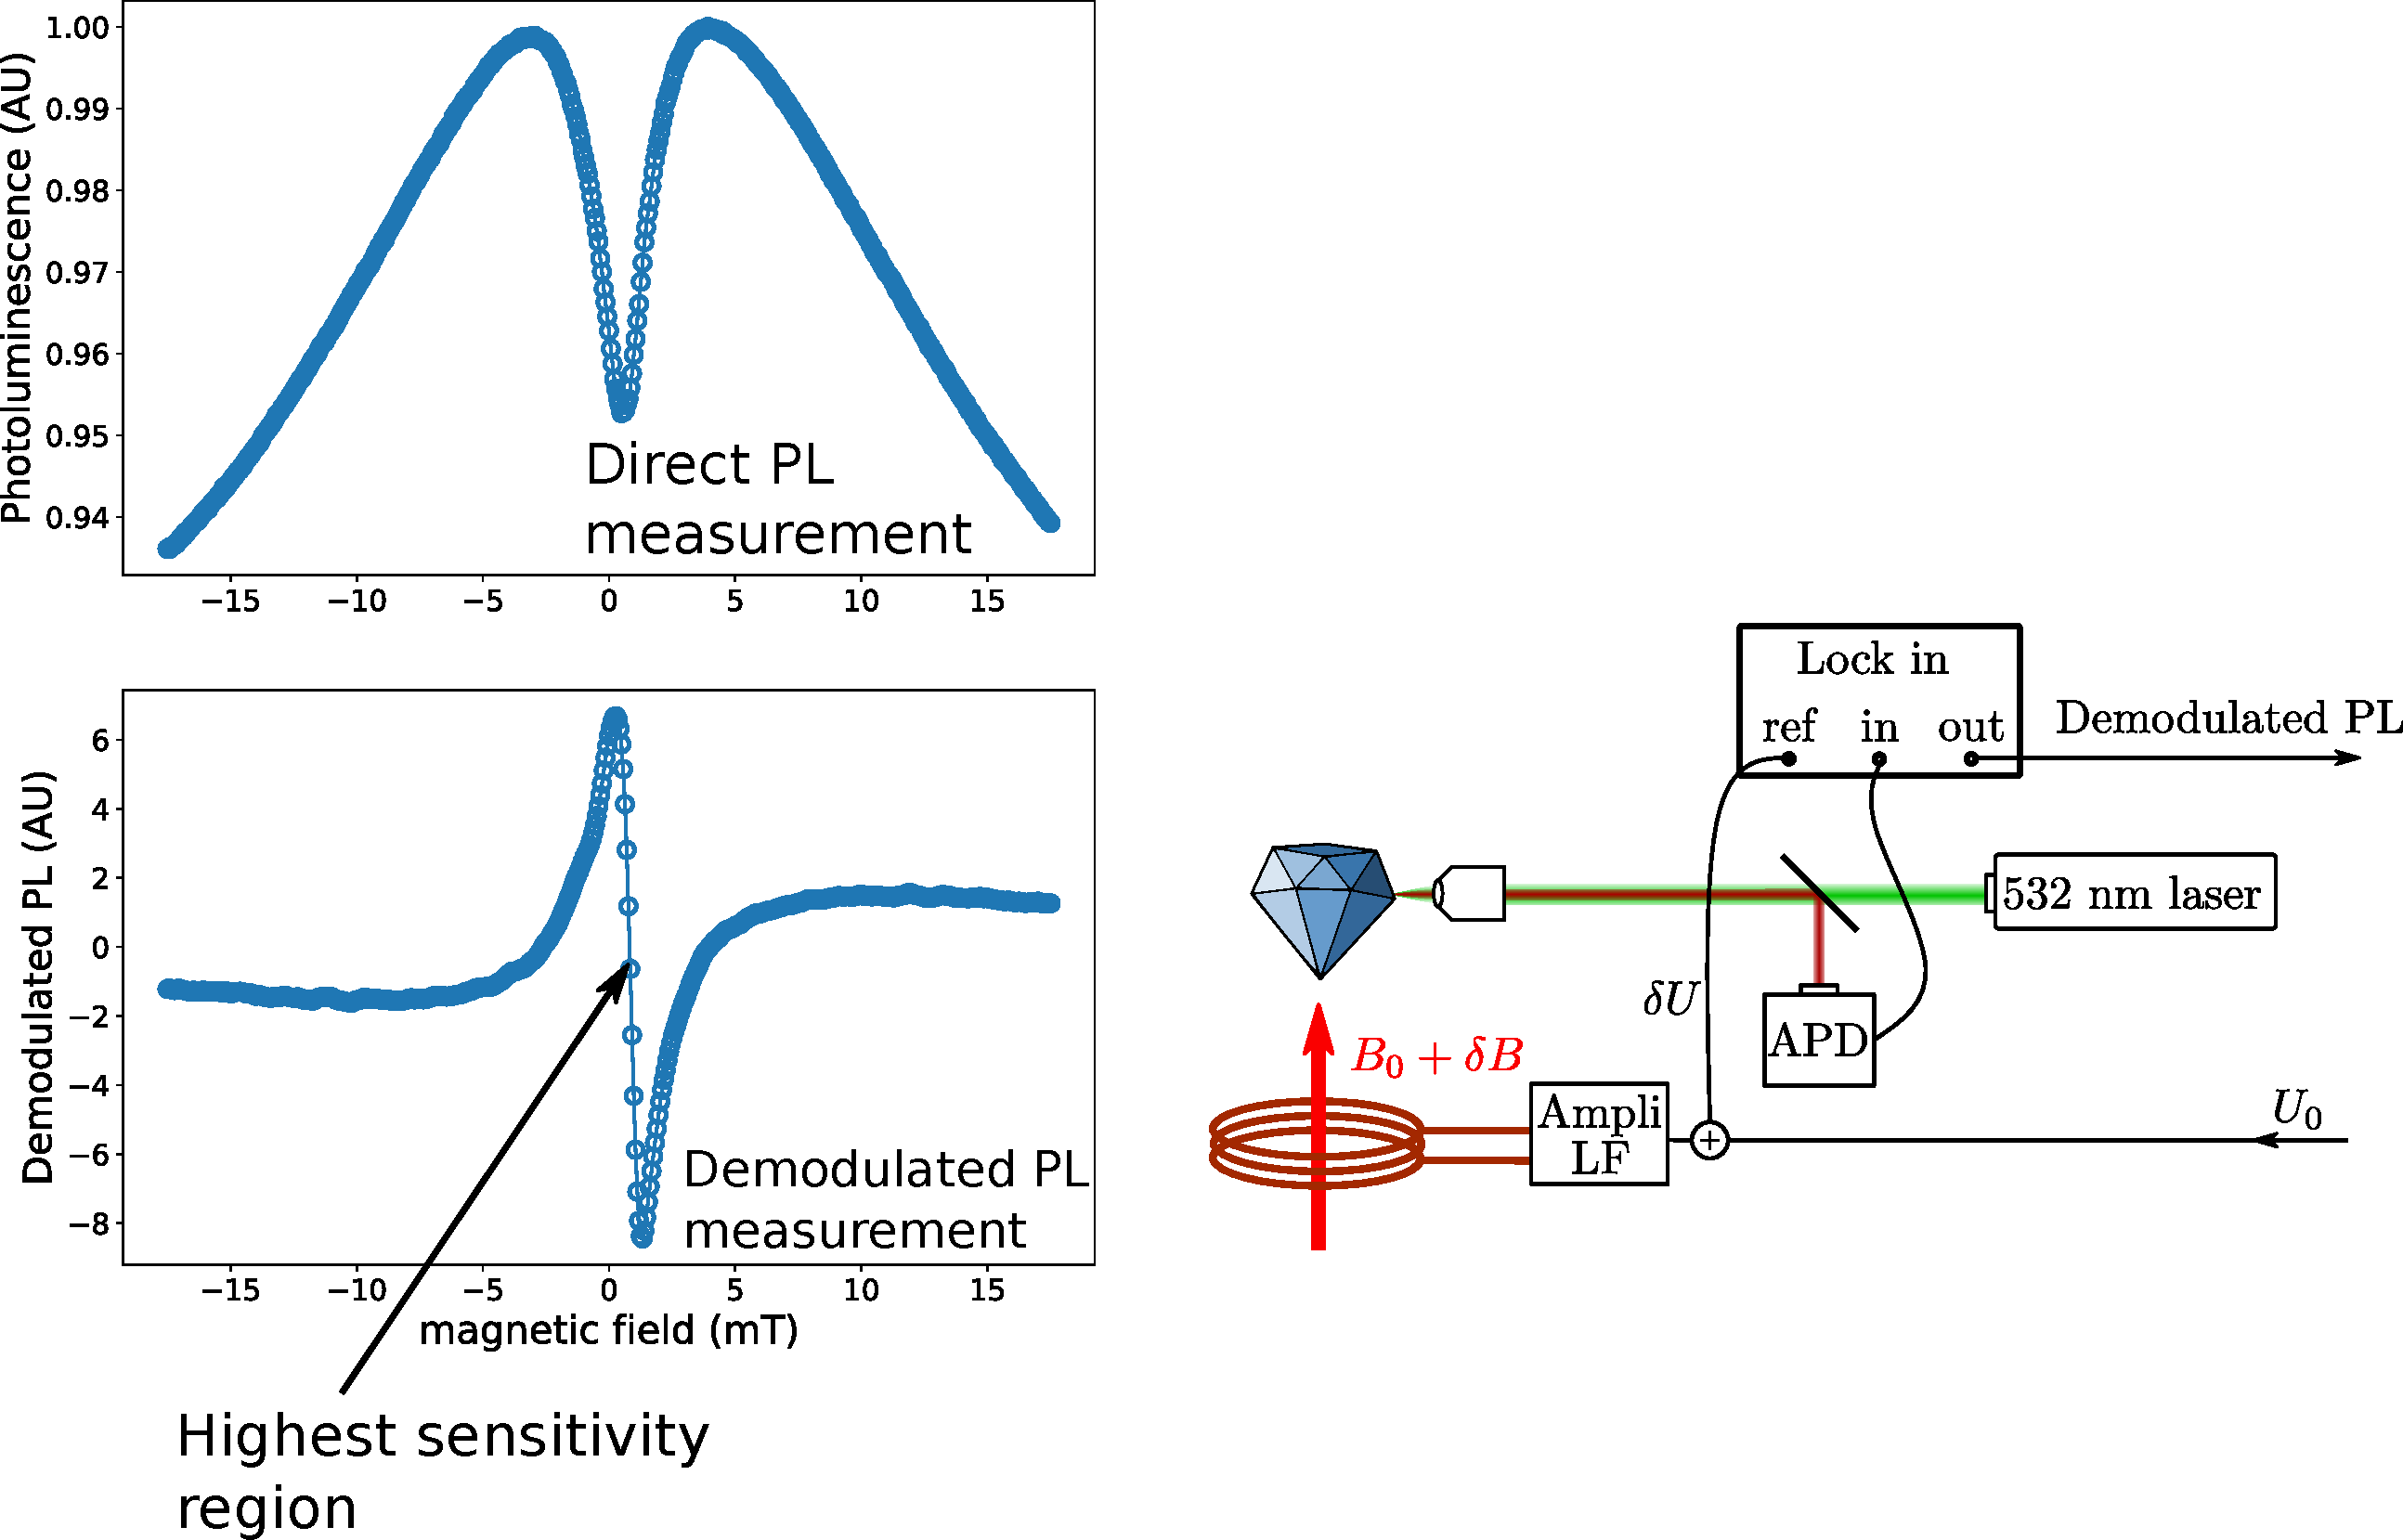
\includegraphics[width=\textwidth,height=0.9\textheight,keepaspectratio]{Slide magneto 1}
\end{frame}
\begin{frame}{Magnetometry protocol}
\centering
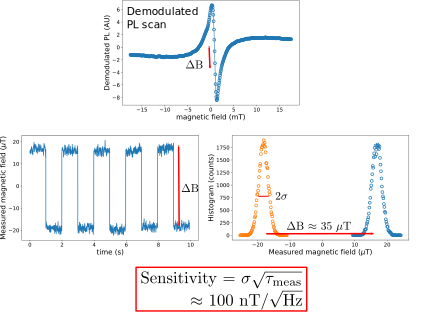
\includegraphics[width=\textwidth,height=0.9\textheight,keepaspectratio]{Slide magneto 2}
\end{frame}
\begin{frame}{Effects of the various effects on the sensitivity}
\centering
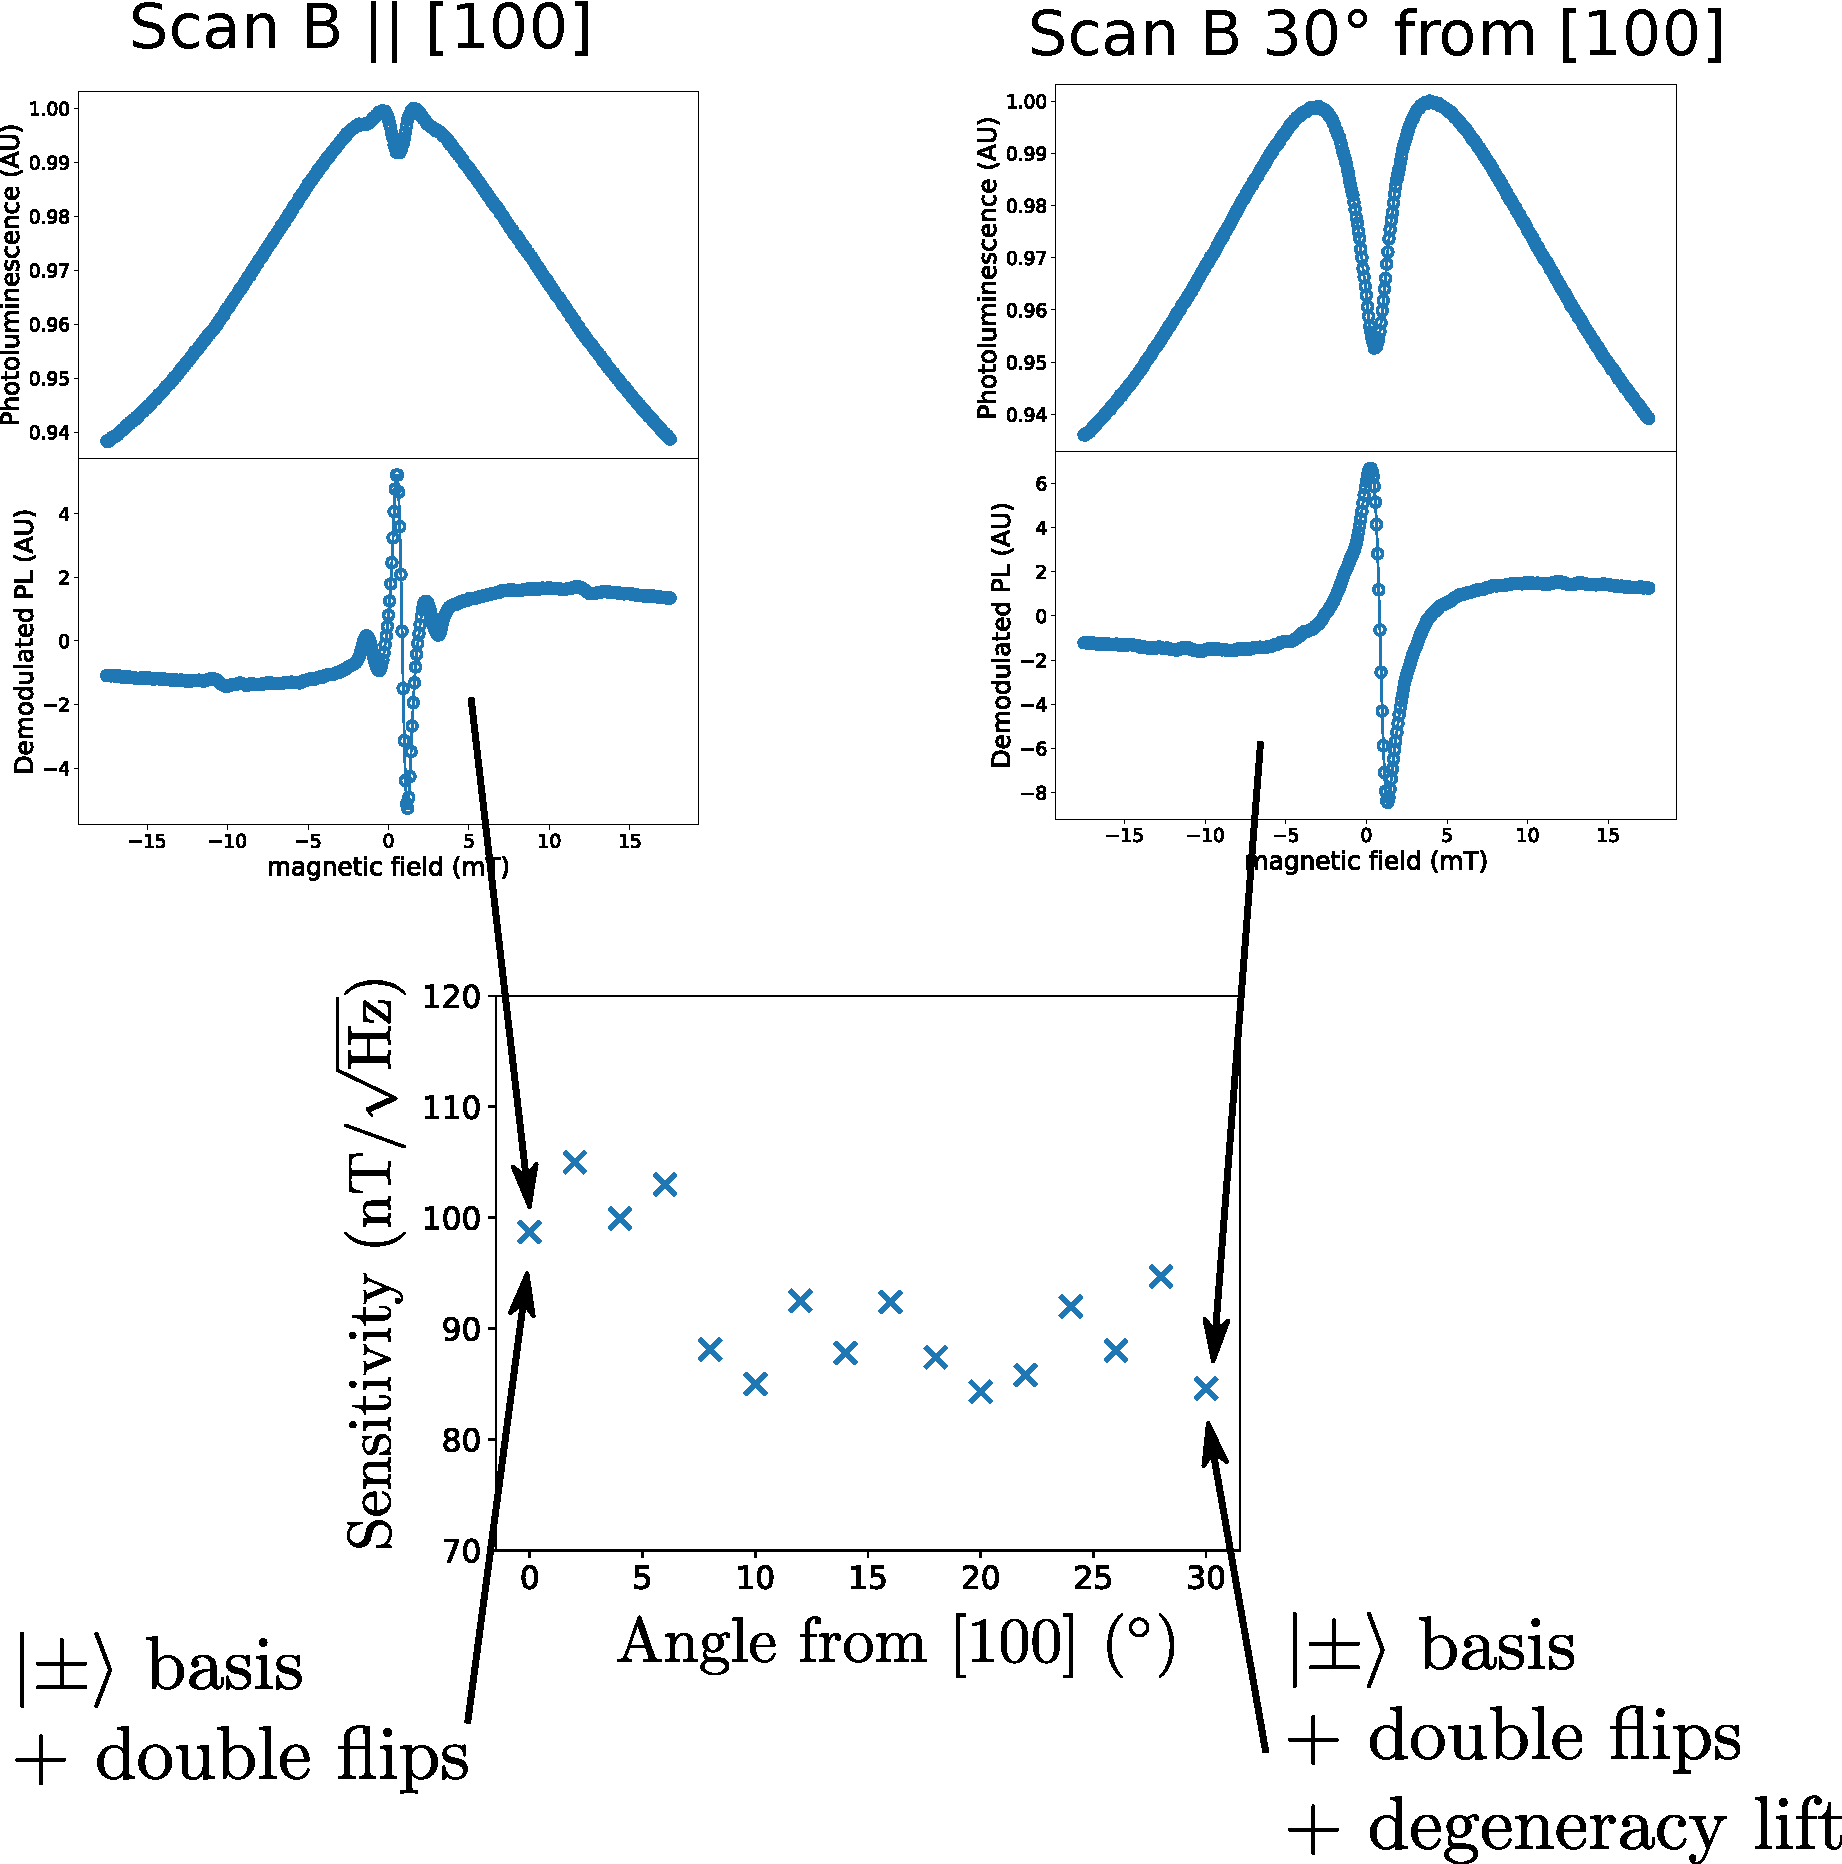
\includegraphics[width=\textwidth,height=0.9\textheight,keepaspectratio]{Slide magneto 3}
\end{frame}
\end{document}